\chapter{Results}\label{chap:results}

\section{ICMP: Ping}\label{sec:res-icmp}

The obvious filter for \texttt{ping -c 4 google.com} is \texttt{icmp}, but it would show nothing here: \texttt{google.com} was resolved to an IPv6 address, so the ping used ICMPv6. With \texttt{icmp or icmpv6}, the four echo requests and replies appear (Figure~\ref{fig:ping}). They share the identifier \texttt{0x8cf7} and are matched by sequence number. The requests leave with hop limit 64 (the IPv6 name for TTL) and the replies arrive with 111. The round-trip times calculated from the time stamps are between 9.5 and 12.0\,ms, about 11.2\,ms on average. The Ethernet destination of each request is the MAC address of our router, not that of Google: the link layer only moves the frame to the next hop. Below the pings, ICMPv6 Neighbor Solicitation and Advertisement messages (orange) are the IPv6 counterpart of ARP.

\begin{figure}[ht]
	\centering
	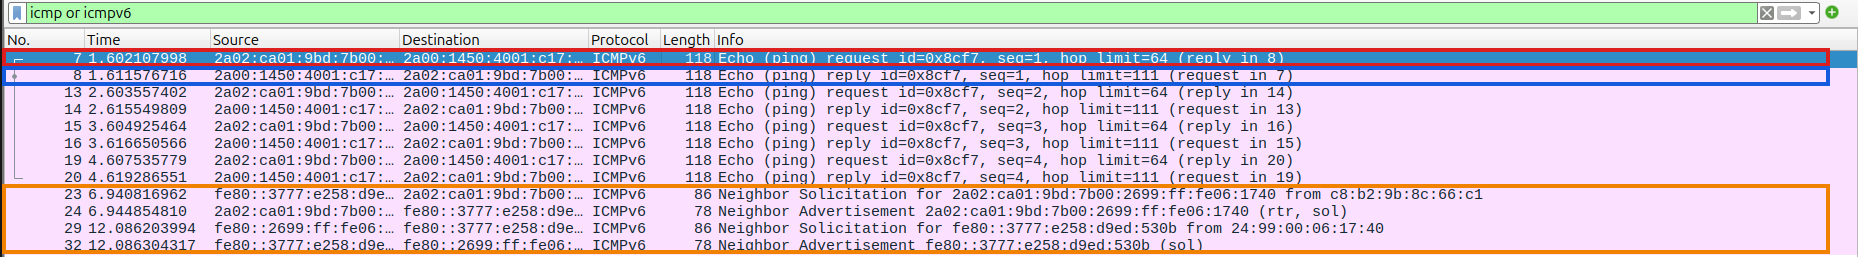
\includegraphics[width=\linewidth]{fig_ping.png}
	\caption{Filter \texttt{icmp or icmpv6}. Red: first echo request, blue: its reply, orange: neighbor discovery.}
	\label{fig:ping}
\end{figure}

\section{DNS Query and Response}\label{sec:res-dns}

The filter \texttt{dns} leaves 78 of the 3\,921 captured packets (Figure~\ref{fig:dns}). The laptop sends its queries to the home router (192.168.178.1), which forwards them upstream. Each query is a UDP datagram from a random source port (here 50773) to port 53, and the answer returns from port 53 and carries the same transaction ID (\texttt{0x9cc3} and \texttt{0xa362}). \texttt{nslookup} asks for both record types. The A query for \texttt{primevideo.com} was answered after 17.9\,ms with four IPv4 addresses (18.66.102.x). The AAAA query was answered after 11.2\,ms, but without an address, only with a start-of-authority (SOA) record: the name simply had no IPv6 address. Oddly, the queries still travel over IPv4 even though the laptop has working IPv6.

\begin{figure}[ht]
	\centering
	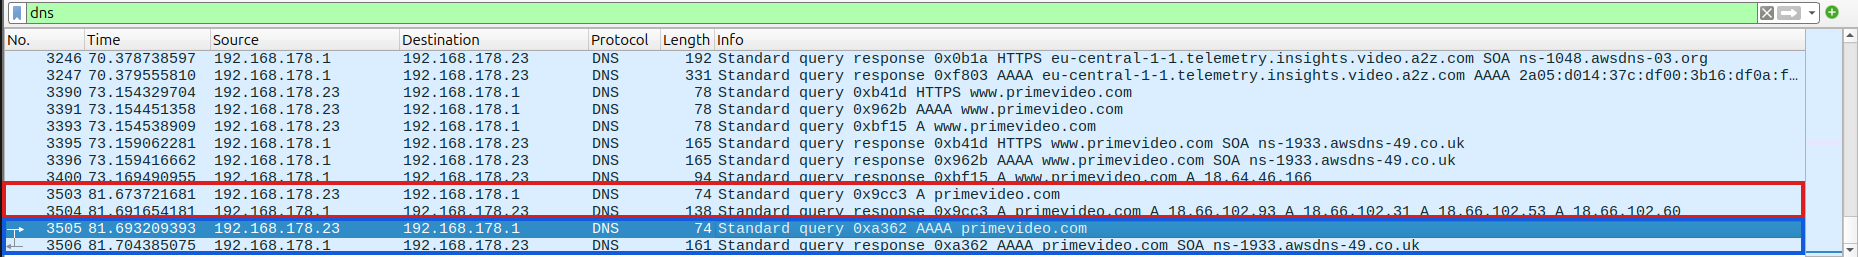
\includegraphics[width=\linewidth]{fig_dns.png}
	\caption{Filter \texttt{dns}. Red: A query and response, blue: AAAA query and response.}
	\label{fig:dns}
\end{figure}

\section{TCP Three-Way Handshake}\label{sec:res-tcp}

For the handshake, we looked at the connection of \texttt{curl} to \texttt{neverssl.com} (TCP stream 0), a deliberately unencrypted site. The filter \texttt{tcp.flags.syn == 1 or tcp.flags.ack == 1 and tcp.stream eq 0} contains a trap: \texttt{and} binds more strongly than \texttt{or}, so it shows \emph{every} SYN in the capture plus the ACKs of stream 0. That is why IPv4 attempts show up in Figure~\ref{fig:tcp}; adding parentheses gives a cleaner view.

\begin{figure}[ht]
	\centering
	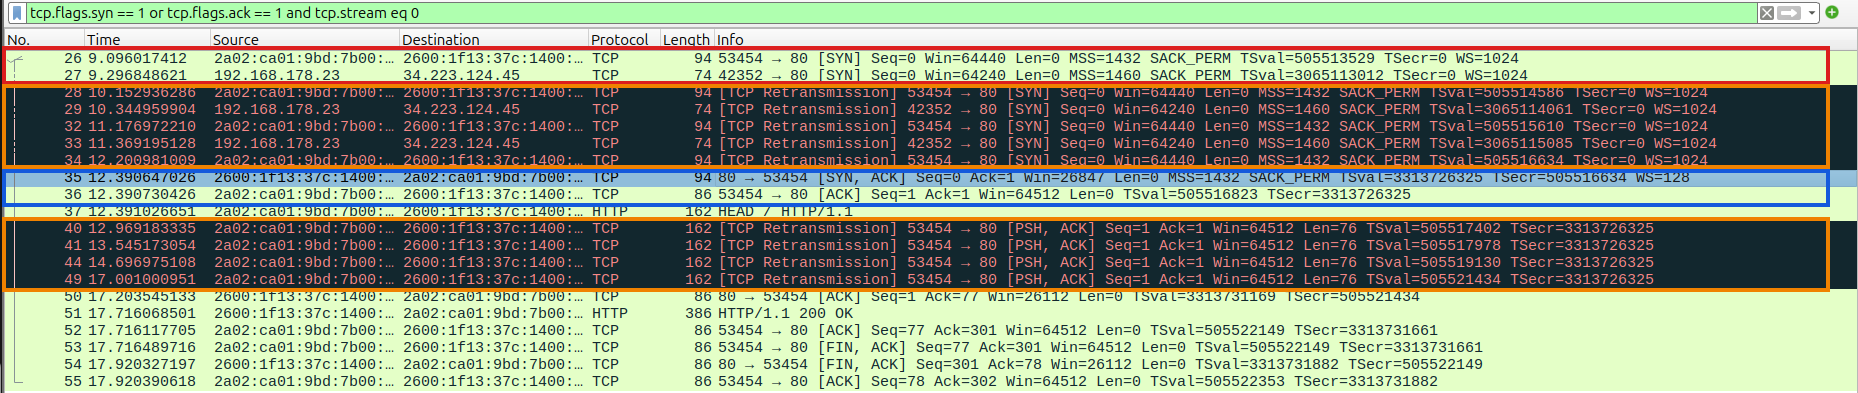
\includegraphics[width=\linewidth]{fig_tcp.png}
	\caption{TCP stream 0. Red: first SYNs (IPv6 and IPv4), orange: retransmissions, blue: SYN-ACK and ACK.}
	\label{fig:tcp}
\end{figure}

The handshake consists of frames 26 (SYN), 35 (SYN-ACK) and 36 (ACK). Wireshark shows relative sequence numbers: \texttt{Seq=0}, then \texttt{Seq=0, Ack=1}, then \texttt{Seq=1, Ack=1}. The acknowledgment is one higher because a SYN consumes one sequence number. The SYN also carries options such as a maximum segment size of 1432 bytes and a window scale of 10 (a multiplier of 1024).

The capture also shows something a textbook diagram leaves out. The IPv6 SYN was sent at 9.1\,s, but the SYN-ACK arrived only at 12.4\,s, after three retransmissions of the SYN at intervals of about one second. Later, the HTTP request itself was retransmitted four times with roughly doubling intervals (0.58 up to 2.3\,s) before the server acknowledged it. We cannot tell from the capture whether Wi-Fi, the access network or the server was responsible, but it shows why TCP numbers its data and retransmits. We also noticed a pair of IPv6 and IPv4 SYNs only about 200\,ms apart (frames 26 and 27). \texttt{curl} had started an IPv6 connection and a fallback over IPv4 (Happy Eyeballs~\cite{rfc8305}), and only the IPv6 attempt completed.

\section{Encapsulation and HTTP}\label{sec:res-encap}

Figure~\ref{fig:layers} expands all layers of the first SYN (frame 26, 94 bytes). The line \texttt{Protocols in frame: eth:ethertype:ipv6:tcp} summarizes the nesting from Figure~\ref{fig:encap}. The Ethernet header holds the MAC addresses (our adapter and the router) and the type \texttt{0x86dd} for IPv6. The IPv6 header holds the 128-bit addresses and the hop limit. The TCP header holds the ports (53454 to 80) and the flags, here only SYN. The sizes add up: $14 + 40 + 40 = 94$ bytes.

\begin{figure}[ht]
	\centering
	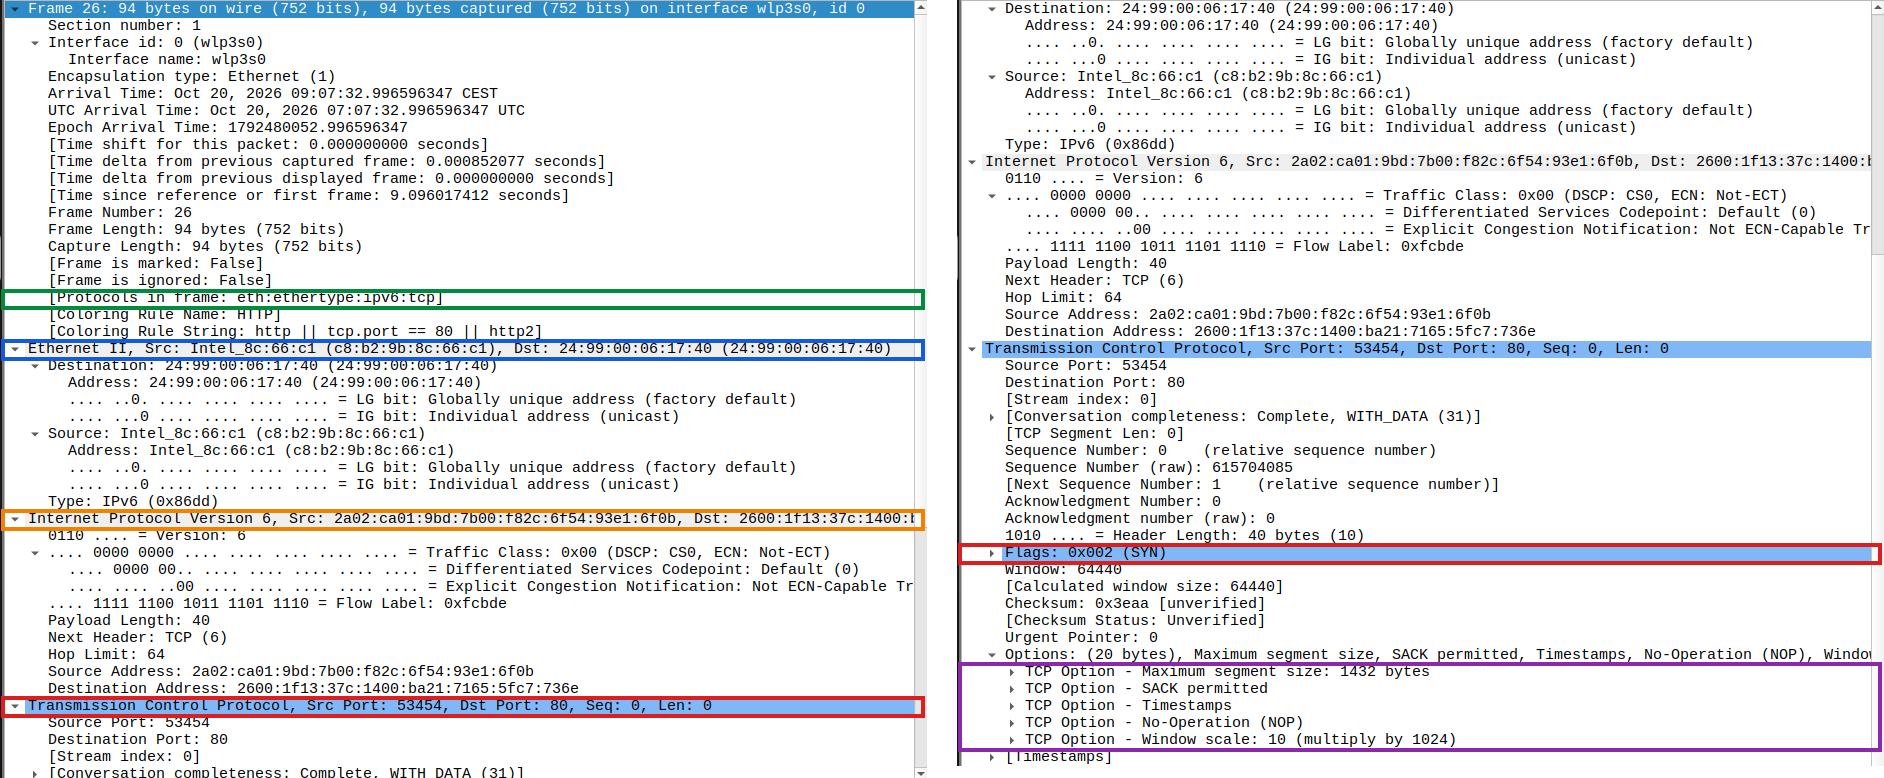
\includegraphics[width=\linewidth]{fig_layers.png}
	\caption{Frame 26 expanded. Left: protocol summary line (green), Ethernet II (blue), IPv6 (orange), TCP (red). Right: TCP flags (red) and options (purple).}
	\label{fig:layers}
\end{figure}

The same stream carries the application layer. \emph{Follow TCP Stream} (Figure~\ref{fig:http}) shows the whole conversation in readable text: a \texttt{HEAD / HTTP/1.1} request with \texttt{Host: neverssl.com} and \texttt{User-Agent: curl/8.5.0}, and a \texttt{200 OK} response from an Apache server. Anyone on the path can read this, including the server software and the client program, which is why HTTPS is the default today.

\begin{figure}[ht]
	\centering
	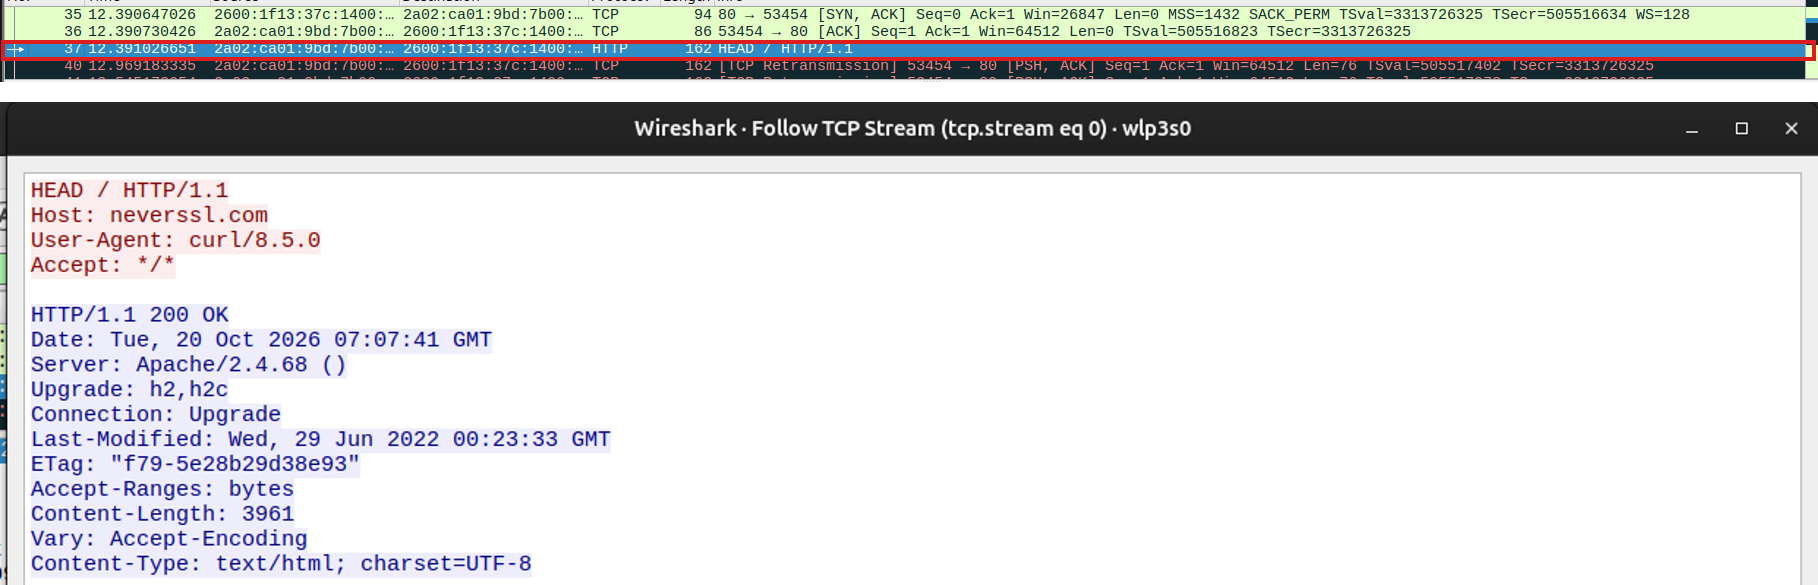
\includegraphics[width=0.92\linewidth]{fig_http.png}
	\caption{The HTTP request (red) and the readable conversation in \emph{Follow TCP Stream}.}
	\label{fig:http}
\end{figure}

\section{HTTPS and TLS}\label{sec:res-tls}

For HTTPS, we ran \texttt{curl https://google.com} and filtered on \texttt{tls}. The connection starts with a Client Hello (frame 20, Figure~\ref{fig:tlshello}), which is still readable: it reveals the server name in the \texttt{server\_name} extension (SNI: \texttt{google.com}), the offered protocols (\texttt{h2} and \texttt{http/1.1}) and the supported TLS versions (1.3 and 1.2). The Server Hello followed 18.6\,ms later. From there on, everything is encrypted. In TLS 1.3, even the certificate and the rest of the handshake are encrypted, so Wireshark labels them \enquote{Application Data}, and the content cannot be recovered without the session keys. The metadata (addresses, ports, sizes, timing and the SNI) remains visible.

\begin{figure}[ht]
	\centering
	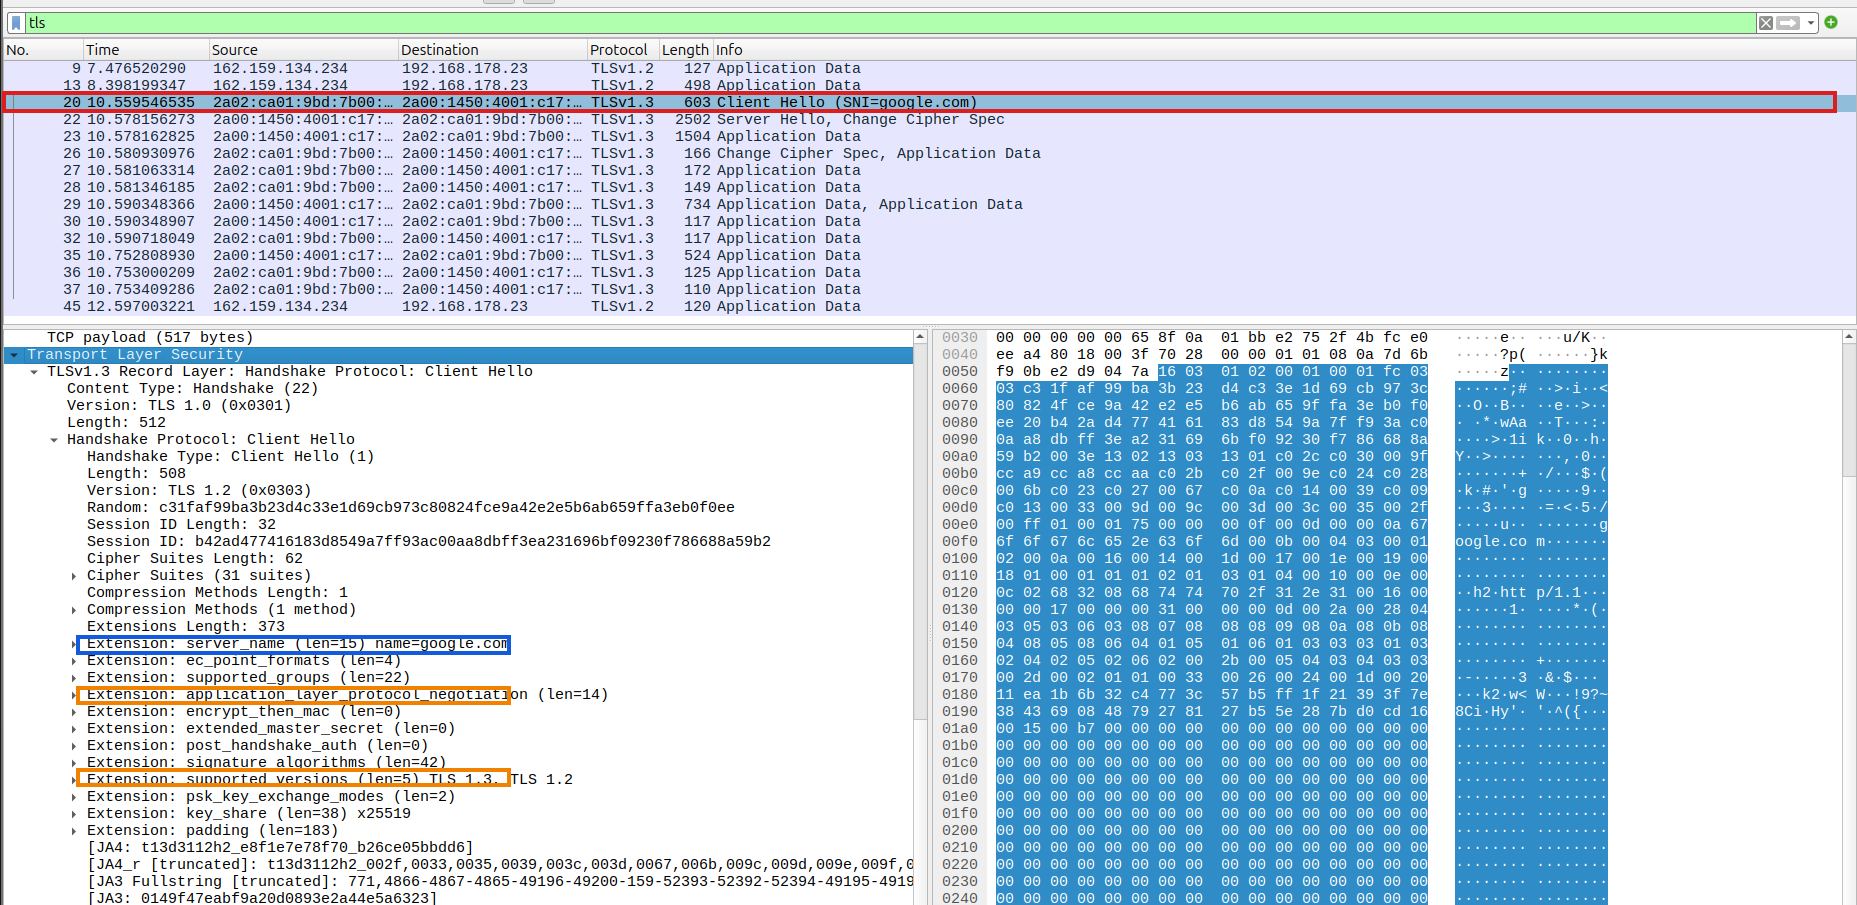
\includegraphics[width=\linewidth]{fig_tls_hello.png}
	\caption{TLS Client Hello. Red: the packet, blue: server name, orange: ALPN and supported versions.}
	\label{fig:tlshello}
\end{figure}
